%!TEX root = main.tex

\section{Dataset and Methodology}
\label{sec:dataset}

We begin this section with the description of packet-level data collection of a mobile voice search service, and then briefly introduce our analysis methodology.

\subsection{Data Collection}

\begin{figure}[th]
	\centering
	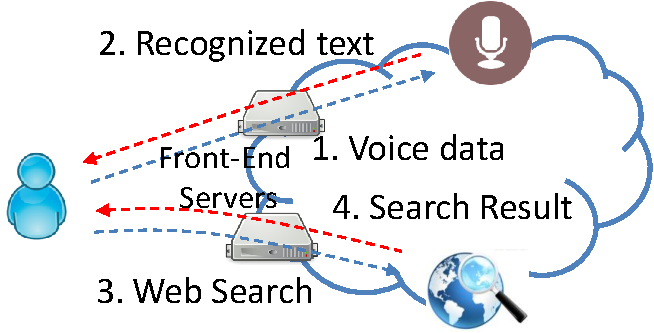
\includegraphics[width=0.8\linewidth]{voice_search_process}
	\caption{Voice search engine infrastructure.}
	\label{fig:voice_search}
\end{figure}

We collect mobile voice search data from one of the top 3 search service providers in China. It serves more than 400 million people per day. A voice search initialized from a mobile terminal consists of two successive phases as shown in Figure~\ref{fig:voice_search}: \emph{voice recognition} (\ie recognize speech to query text) and \emph{web search} (i.e. search with returned query text). Voice recognition and web search are served by two types of servers via standard HTTP protocol. As such, a voice search session consists of two TCP flows.

We collect packet-level traces from front-end servers of both voice recognition and web search by sampling flows uniformly at random, resulting in two datasets that correspond to the two phases of voice search. The front-end servers where we obtained datasets provide services for mobile users of the same geographical locations. Thus, we can safely assume flows in the two datasets transferring through network with similar network characteristics. The web search servers provide search services for both voice search and traditional user-type search. The datasets were collected from in April 2015 for two weeks. In total, we obtained about 1 million voice recognition flows and 3 million web search flows. We report measurement results for each of the two phases of voice search.

All the voice search requests are from mobile apps, especially from Android platform, either via cellular network or WiFi network. About 2.5\% of the voice recognition flows and 6.7\% of the web search flows are from cellular network, which is constituted by a mixture of 2.5G, 3G and 4G network\footnote{The cellular network type was inferred using the HTTP header field ``x-up-bear-type''.}. However, we observed a very limited number of 2.5G and 4G flows (less than 0.5\% of the total flows) in our datasets\footnote{4G network is in the initial deployment in China and has a limited coverage.} and thus omit them from analysis. In total, they make up about 2.5\% of the flows.


\begin{figure}[th]
\centering
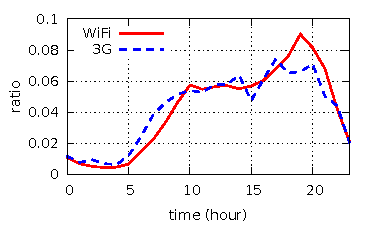
\includegraphics[width=0.8\linewidth]{voice_time_rate}
\caption{Distribution of voice search requests in a day.}
\label{fig:voice_time_rate}
\end{figure}

Figure~\ref{fig:voice_time_rate} shows the distribution of voice search flows over time of a day. Flows are binned into 1-hour frame and the ratio of flows in each bin to the flows of a day is reported. Not surprisingly, we observe a sharp raise of the search volume from 5AM to 10AM. The search volume from 3G network remains relatively stable in the day time and declines around 10PM, while we observe continuous growth of the WiFi search which reaches the peak of day at 7PM. The daily trend for web search flows is similar and thus not show. In fact, the daily search volume variation trend we observed is very similar to that report in \cite{Song:2013:EEU:2488388.2488493} for Bing mobile search, showing that our datasets are indeed representative.

\subsection{TCP Performance Metrics}

For a voice search session, both the voice recognition phase and web search phase contribute to the performance. However, they could have very distinct behavior from the serve-side view. This is because, in the voice recognition phase, server acts as TCP receiver, while in the web search phase, server is TCP sender. Note that TCP is a sender-driven transmission protocol and its transmission performance is basically affected by the efficiency that sender could handle congestion events, as well as the capability that receiver could receive data.

We examine the TCP performance factors of each phase for individual voice search sessions and their impacts on the flow \emph{finish time}. The finish time of a TCP flow measures the duration from the time when client initiates the connection till the time when the last byte of data is acknowledged. As the exact time when client initializes SYN packet is not available at server side, we mark the time when serve received the SYN packet as the start of the duration. It is also noteworthy that since we are interested in the network-related performance, the finish time of a voice recognition flow excludes the time consumed by servers to translate voice data into text. Likewise, the finish time of a web search flow excludes the time consumed by servers to get the search results from data centers for web search flows. It is also noteworthy that for the web search phase, we only consider flows carrying search results that are dynamically generated by servers based on the query and ignore those corresponding to static content like CSS/JavaScript files for the reasons that the performance of the static content (as opposed to the dynamic search results) can be optimized easily through CDN (Content Delivery Network) caching.

\begin{figure}[ht]
\centering
\begin{subfigure}[b]{0.8\linewidth}
	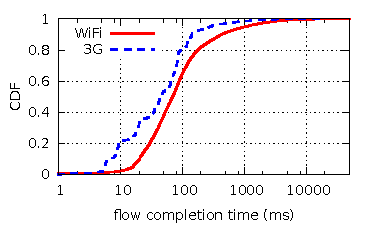
\includegraphics[width=\textwidth]{voice_finish_time}
\caption{Voice recognition}
\label{fig:voice_finish_time}
\end{subfigure} \\
%\vspace{0.1in}
\begin{subfigure}[b]{0.8\linewidth}
	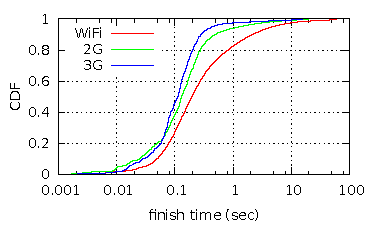
\includegraphics[width=\textwidth]{web_finish_time}
\caption{Web search}
\label{fig:web_finish_time}
\end{subfigure}
\caption{CDFs of finish time in the two phases.}
\label{fig:finish_time}
\end{figure}


Figure~\ref{fig:finish_time} plots the cumulative distribution (CDF) of the finish time of TCP flows in the two phases. Interestingly, we find that in both phases 3G flows experience a shorter finish time than WiFi flows. Furthermore, some flows experience an extraordinarily long finish time compared with others, showing a heavy tail behavior that was also found in Google search \cite{flach2013reducing}. For example, while most of the voice recognition flows finish in 0.1 second, a non-negligible fraction of flows (5\% in WiFi, and 2\% in 3G) take more than 1 second to upload the voice data. 

%Figure~\ref{fig:web_finish_time} shows the CDF of finish time of web search flows. In the figure, the overall finish time of flows in 2G and 3G (with median values 0.013s and 0.011s) in also shorter than that of flows in WiFi network (with median value 0.2s). More than 25\% of flows in all networks experience finish time less than 0.1 second. However, 5\% of flows in 2G network and 18\% in WiFi network experience finish time more than 1 second. Furthermore, about 3\% of flows in WiFi network are with finish time more than 10 seconds, which is a great performance degradation.

A comparison of the TCP flow finish time between voice recognition and web search in Figure~\ref{fig:finish_time} shows that the finish time in web search contribute to the majority of the user perceived (network-related) performance of a voice search session. However, it by no means indicates that understanding the performance of voice recognition flows is not as important as that of web search flows. This is because voice recognition is the first step of the whole voice search process and a long recognition time would certainly result in bad user experience, even early quit of the process. We were motivated by these observations to have an in-depth analysis of the TCP performance and its impact on the flow finish time in each phase of mobile voice search.

% some of voice recognition flows suffer from timeout retransmission, which is a great performance degradation~\cite{flach2013reducing}. Second, a non-negligible fraction of voice recognition flows are terminated before voice data transmission completes. These bad user experiences also inspire us to understand what factors and how they impact user-perceived performance in voice recognition flows.


%To evaluate the impact of network quality on user experience in voice search, we mainly consider the following network factors in the analysis:
In particular, we consider the following TCP performance factors. 

\begin{itemize}
	\item {Round Trip Time (RTT): } RTT is a commonly used indicator of TCP performance, especially for short TCP flows like search flows.
	
	\item {Number of lost/disordered packets: } Both packet loss and packet reordering could affect the transmission efficiency. Packet loss leads to reduction of sender's congestion window. Although packet reordering does not reduce congestion window, it can prevent congestion window from growing and may trigger spurious retransmission. 
	
	\item {Timeout Retransmission: } The TCP sender has to wait for a RTO (Retransmission Timeout) before retransmitting the lost packet. The RTO can be tens of or hundreds of RTTs. Such kind of ``expensive'' retransmissions can degrade the TCP performance, especially for short flows (like those considered in this paper)~\cite{flach2013reducing}. We refer such kind of retransmissions as timeout retransmissions in this paper.

	
\end{itemize}

When examining the impact of the above factors on TCP finish time, we also consider the potential impact of TCP flow size. We are particular interested in the disparity that might exist when issuing voice searches from 3G and WiFi. 